\documentclass[11pt,answers]{exam} %noanswers
\usepackage{multicol}
\usepackage[usenames]{color} %used for font color
\usepackage{amssymb} %maths
\usepackage{amsmath} %maths
\usepackage[utf8]{inputenc} %useful to type directly diacritic characters
\usepackage{siunitx}
\usepackage{mathtools}
\usepackage{float}
\usepackage[version=4]{mhchem}
\newcommand{\qtty}[2]{\left(\qty{#1}{#2}\right)}
\sisetup{display-per-mode = symbol }
\sisetup{inter-unit-product = \ensuremath { { } \cdot { } } }
\usepackage[letterpaper, total={7in, 10in}]{geometry}
\usepackage{graphicx} % Required for inserting images
\renewcommand{\epsilon}{\varepsilon}
\renewcommand{\vec}[1]{\mathbf{#1}}
\newcommand{\mat}[1]{\begin{bmatrix*}[r] #1 \end{bmatrix*}}

\begin{document}
\flushleft
Name:\ \makebox[4in]{\hrulefill} \hspace{1in} Date:\ \makebox[1in]{\hrulefill}
\begin{center}
    \textbf{\S 1.8 Introduction to Linear Transformations}
\end{center}


\begin{questions}
    \question Let $A = \mat{2 & 0 \\ 0 & 2}$, and define $T : \mathbb{R}^2 \rightarrow \mathbb{R}^2$ by $T\left(\vec{x}\right) = A\vec{x}$. Find the images under $T$ of $\vec{u}=\mat{1 \\ -3}$ and $\vec{v}=\mat{a \\ b \\ c}$.
    \question Let $A = \mat{0.5 & 0 & 0 \\ 0 & 0.5 & 0 \\ 0 & 0 & 0.5}$, and define $T : \mathbb{R}^3 \rightarrow \mathbb{R}^3$ by $T\left(\vec{x}\right) = A\vec{x}$. Find the images under $T$ of $\vec{u}=\mat{1 \\ 0 \\ -4}$ and $\vec{v}=\mat{a \\ b}$.
    \begin{center}\rule{4in}{0.1mm}\end{center}
    \uplevel{With $T$ defined by $T\left(\vec{x}\right) = A\vec{x}$, find a vector $\vec{x}$ whose image under $T$ is $\vec{b}$ and determine whether $\vec{x}$ is unique.}
    \question $A=\mat{ 1 & 0 & -2 \\ -2 & 1 & 6 \\ 3 & -2 & -5}, \vec{b}=  \mat{-1 \\ 7 \\ -3}$
    \question $A=\mat{ 1 & -3 & 2 \\ 0 & 1 & -4 \\ 3 & -5 & -9}, \vec{b} = \mat{6 &\\ -7 \\ -9}$
    \question $A = \mat{1 & -5 & -7 \\ -3 & 7 & 5}, \vec{b}= \mat{ -2 \\ -2 }$
    \question $A = \mat{1 & -2 & 1 \\ 3 & -4 & 5 \\ 0 & 1 & 1 \\ -3 & 5 & -4}, \vec{b} = \mat{1 \\ 9 \\ 3 \\ -6}$
    \question Let $A$ be a $6\times 5$ matrix. What must $a$ and $b$ by in order to define  $T:\mathbb{R}^a \rightarrow \mathbb{R}^b$ by $T\left(\vec{x}\right) = A\vec{x}$?
    \question How many rows and how many columns must a matrix $A$ have in order to define a mapping from $\mathbb{R}^5$ into $\mathbb{R}^4$ by the rule $T(\vec{x}) = A\vec{x}$?
    \begin{center}\rule{4in}{0.1mm}\end{center}
    \uplevel{Find all $\vec{x}$ in $\mathbb{R}^4$ that are mapped into the zero vector by the transformation $\vec{x}\mapsto A\vec{x}$ for the given matrix $A$.}
    \question $A = \mat{1 & -4 & 7 & -5 \\ 0 & 1 & -4 & 3 \\ 2 & -6 & 6 & -4}$
    \question $A = \mat{1 & 3 & 9 & 2 \\ 1 & 0 & 3 & -4 \\ 0 & 1 & 2 & 3 \\ -2 & 3 & 0 & 5}$
    \question Let $\vec{v} = \mat{-1 \\ 1\\ 0}$, and let $A$ be the matrix in Exercise 9. Is $\vec{v}$ in the range of the linear transformation $\vec{x}\mapsto A\vec{x}$? Why or why not?
    \question Let $\vec{b} = \mat{-1 & 3 & -1 & 4}$, and let $A$ be the matrix in Exercise 10. Is $\vec{b}$ in the range of the linear transformation $\vec{x}\mapsto A\vec{x}$? Why or why not?
    \begin{center}\rule{4in}{0.1mm}\end{center}
    \uplevel{Use a rectangular coordinate system to plot $\vec{u}=\mat{5 \\ 2}, \vec{v}=\mat{-2 \\ 4}$, and their images under the given transformation $T$. Describe geoemetrically what $T$ does to each vector in $\mathbb{R}^2$.}
    
    
        \question $T(\vec{x}) = \mat{-1 & 0 \\ 0 & -1} \mat{x_1 \\ x_2}$    
        \begin{figure}[H]
            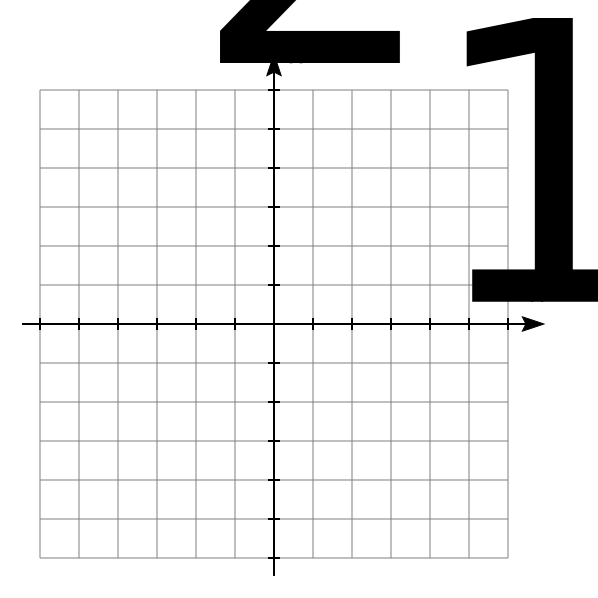
\includegraphics[width=5cm]{blank6x6}
        \end{figure}
        
         \question $T(\vec{x}) = \mat{0.5 & 0 \\ 0 & 0.5} \mat{x_1 \\ x_2}$
        \begin{figure}[H]
            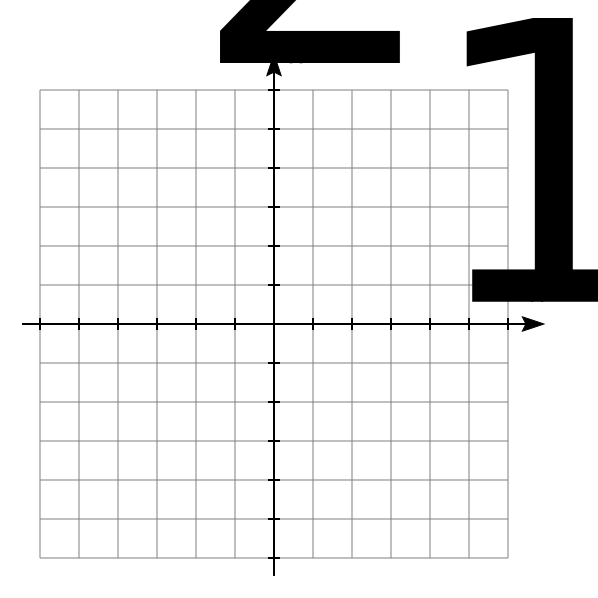
\includegraphics[width=5cm]{blank6x6}
        \end{figure}
        \pagebreak
        \question $T(\vec{x}) = \mat{0 & 0 \\ 0 & 1} \mat{x_1 \\ x_2}$
        \begin{figure}[H]
            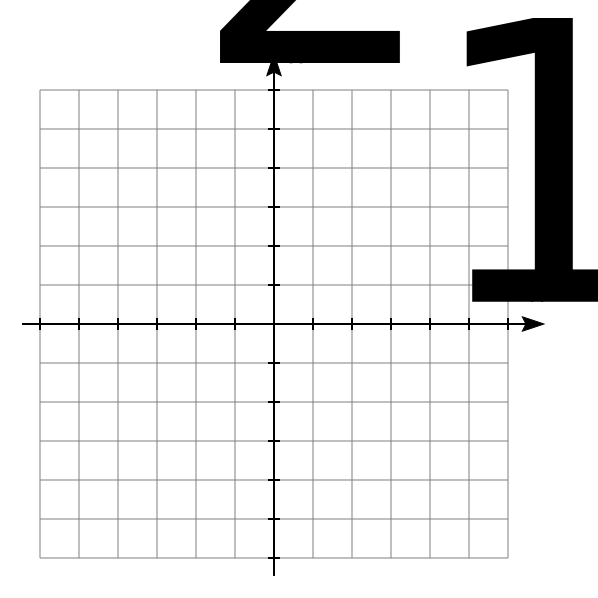
\includegraphics[width=5cm]{blank6x6}
        \end{figure}
        \question $T(\vec{x}) = \mat{0 & 1 \\ 1 & 0} \mat{x_1 \\ x_2}$
        \begin{figure}[H]
            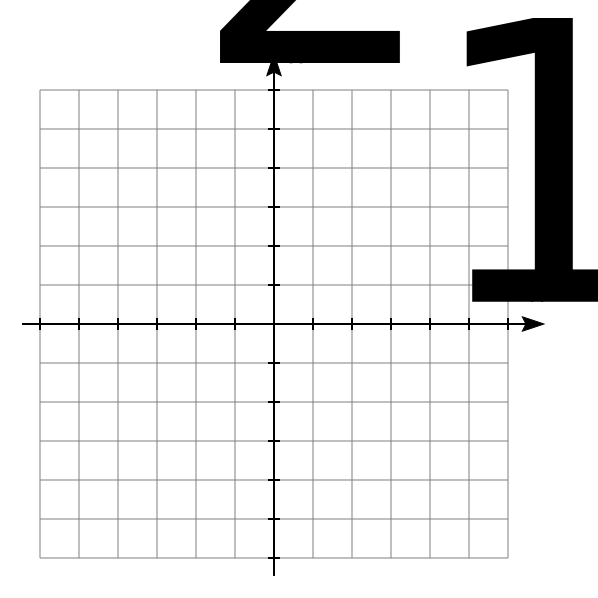
\includegraphics[width=5cm]{blank6x6}
        \end{figure}
    
    \question Let $T : \mathbb{R}^2 \rightarrow \mathbb{R}^2$ be a linear transformation that maps $\vec{u} = \mat{5 \\ 2}$ into $\mat{2 \\ 1}$ and maps $\vec{v} = \mat{1 \\ 3}$ into $\mat{-1 & 3}$. Use the fact that $T$ is a \emph{linear} transformation to find the images under $T$ of $3\vec{u}$, $2\vec{v}$, and $3\vec{u}+2\vec{v}$.
    \question insert
    \question Let $\vec{e}_1 = \mat{1\\0}, \vec{e}_2 = \mat{0\\1}, \vec{y}_1=\mat{2\\5}, \vec{y}_2=\mat{-1\\6}$, and let $T:\mathbb{R}^2\rightarrow\mathbb{R}^2$ be a linear transformation that maps $\vec{e}_1$ into $\vec{y}_1$ and maps $\vec{e}_2$ into $\vec{y}_2$. Find the images of $\mat{5\\-4}$ and $\mat{x_1 \\ x_2}$.
    \question Let $\vec{x} = \mat{x_1 \\ x_2}, \vec{v}_1 = \mat{-2 \\ 5}, \vec{v}_2 = \mat{7\\-3}$, and let $T:\mathbb{R}^2\rightarrow \mathbb{R}^2$ be a linear transformation that maps $\vec{x}$ into $x_1\vec{v}_1+x_2\vec{x}_2$. Find a matrix $A$ such that $T(\vec{x})$ is $A\vec{x}$ for each $\vec{x}$.

    \begin{center}\rule{4in}{0.1mm}\end{center}
    \uplevel{Mark each statement True or False (\textbf{T}/\textbf{F}). Justify each answer.}
    \question (\textbf{T}/\textbf{F}) A linear transformation is a special type of function.
    \question (\textbf{T}/\textbf{F}) Every matrix transformation is a linear transformation.
    \question (\textbf{T}/\textbf{F}) If $A$ is a $3 \times 5$ matrix and $T$ is a transformation defined by $T(\vec{x}) = A\vec{x}$, then the domain of $T$ is $\mathbb{R}^3$.
    \question (\textbf{T}/\textbf{F}) The codomain of the transformation $\vec{x} \mapsto A\vec{x}$ is the set of all linear combinations of the columns of $A$.
    \question (\textbf{T}/\textbf{F}) If $T : \mathbb{R}^n \rightarrow \mathbb{R}^m$ is a linear transformation and if $\vec{c}$ is in $\mathbb{R}^m$, then a uniqueness question is ``Is $\vec{c}$ in the range of $T$?''
    \question (\textbf{T}/\textbf{F}) Every linear transformation is a matrix transformation.
    \question (\textbf{T}/\textbf{F}) A linear transformation preserves the operations of vetor addition and scalar multiplciation.
    \question (\textbf{T}/\textbf{F}) A linear transformation preserves the operations of vector addition and scalar multiplication.
    \question (\textbf{T}/\textbf{F}) A transformation $T$ is linear if and only if $T\left(c_1\vec{v}_1 + c_2\vec{v}_2\right) = c_1 T(\vec{v}_1) + c_2 T(\vec{v}_2)$ for all $\vec{v}_1$ and $\vec{v}_2$ in the domain of $T$ and for all scalars $c_1$ and $c_2$.
    \question (\textbf{T}/\textbf{F}) The superposition principle is a physical description of a linear transformation.
    \question (\textbf{T}/\textbf{F}) Let $T : \mathbb{R}^2 \rightarrow \mathbb{R}^2$ be the linear transformation that reflecs each point through the $x_1$-axis. (See Practice Problem 2.). Make two sketches similar to Figure 6 that illustrates properties (i) and (ii) of a linear transformation.
    \question (\textbf{T}/\textbf{F}) Suppose vectors $\vec{v}_1, \ldots, \vec{v}_p$ span $\mathbb{R}^n$, and let $T : \mathbb{R}^n \rightarrow \mathbb{R}^n$ be a linear transformation. Suppose $T(\vec{v}_i) = \vec{0}$ for $i=1,\ldots,p$. Show that $T$ is a zero transformation. That is, show that if $\vec{x}$ is any vector in $\mathbb{R}^n$, then $T(\vec{x}) = \vec{0}$.
    \question (\textbf{T}/\textbf{F}) Given $\vec{v}\neq\vec{0}$ and $\vec{p}$ in $\mathbb{R}^n$, the line through $\vec{p}$ in the directin of $\vec{v}$ has the parametric equation $\vec{x}=\vec{p}+t\vec{v}$. Show that a linear transformation $T:\mathbb{R}^n\rightarrow\mathbb{R}^n$ maps this line onto another line or onto a single point (a \emph{degenerate line}).
    \question (\textbf{T}/\textbf{F}) Let $\vec{u}$ and $\vec{v}$ be linearly independent vectors in $\mathbb{R}^3$, and let $P$ be the plane through $\vec{u}$, $\vec{v}$, and $\vec{0}$. The parametric equation of $P$ is $\vec{x}=s\vec{u}+t\vec{v}$ (with $s$, $t$ in $\mathbb{R}$). Show that a linear transformation $T:\mathbb{R}^3 \rightarrow \mathbb{R}^3$ maps $P$ onto a plane through $\vec{0}$, or onto a line through $\vec{0}$, or onto just the origin in $\mathbb{R}^3$. What must be true about $T(\vec{u})$ and $T(\vec{v})$ in order fo rthe image of the plane $P$ to be a plane?
    \question (\textbf{T}/\textbf{F}) 
   
    
\end{questions}
\end{document}